% TECNOLOGIAS-------------------------------------------------------------------

\chapter{TECNOLOGIAS}

%%% Original: Neste capítulo estão descritas as tecnologias aplicadas no decorrer do trabalho.
Este Capítulo descreve as tecnologias necessárias para o desenvolvimento deste trabalho.

\section{API}
%https://www.devmedia.com.br/application-programming-interface-desenvolvendo-apis-de-software/30548
API é o acrônimo de Interface de Programação de Aplicativos. Na grande maioria das vezes uma API se comunica com diversos outros códigos interligando diversas funções em um aplicativo, como pode ser visto na \autoref{fig:api}. Esta interface de programação é um conjunto de padrões de programação que permitem a construção de aplicativos e a sua utilização. Portanto, uma API é uma abstração da funcionalidade e da implementação interna de cada componente. Com uma API é possível criar sistemas melhores e minimizar o entendimento de todos os detalhes de um componente e assim serve como um “alicerce”, abstraindo a funcionalidade e implementação interna de cada componente \cite{jaroslavapi}.

Segundo \citeonline{jaroslavapi}, API é um conjunto de classes, seus métodos e seus campos.
Uma boa API é o conjunto de arquivos que o aplicativo lê ou escreve, bem como seu formato. Algumas aplicações sequer fazem uso do disco rígido, assim sendo não precisam se preocupar com esse tipo de coisa. O primeiro objetivo da engenharia é produzir sistemas funcionais. Uma API também precisa ser fácil de usar, largamente adotada e produtiva.

\begin{figure}[H]
    \centering
    \caption{API -  Estrutura}
    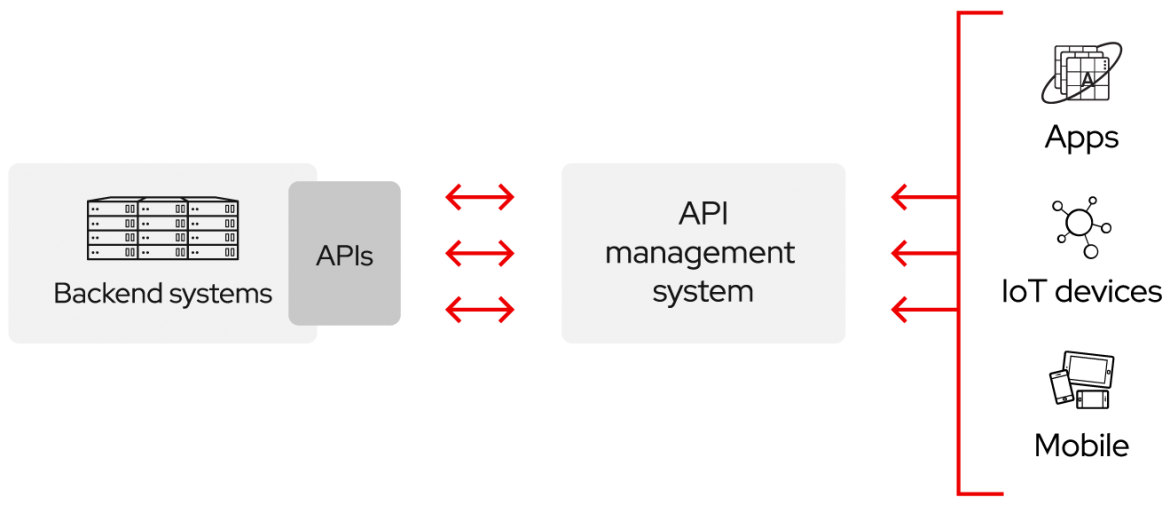
\includegraphics[width=0.8\textwidth]{./dados/figuras/fig10}
    \fonte{\citeonline{redhat}}
    \label{fig:api}
\end{figure}

O World Wide Web Consortium (W3C) é a principal organização de padronização da rede mundial de computadores, desenvolvendo especificações técnicas e orientações através de um processo projetado para maximizar a consenso sobre as recomendações, garantindo qualidades técnicas e editoriais, por meio do desenvolvimento de protocolos comuns e fóruns abertos que promovam a sua evolução e assegurem a sua interoperabilidade, para levar a web ao seu potencial máximo \cite{api:w3c}.

\section{Geolocalização}

%%% Original: A geolocalização é capacidade de informar suas coordenadas e pode conseguir recuperar essas informações através do IP, GPS, conexão de \textit{Wi-Fi}, entre outros. Extremamente útil para uma serie de objetivos como informações sobre um determinado local ou uma rota de navegação, a API de geolocalização consiste em um método para localizar exatamente a posição de um usuário, simples de ser implementada e utilizada. Existem duas formas de realizar a captura da geolocalização através da API W3C, compatível com navegadores em \textit{desktop} ou dispositivos móveis. É necessária a autorização do usuário para acessar as suas informações de geolocalização, pois pode comprometer a sua privacidade e integridade \cite{geolocalizacao:2011}.

%%% Rev-Madalozzo: Neste parágrafo você fala de "API W3C", mas nenhum lugar antes daqui comenta sobre isso. Creio que seria interessante dizer o que é.
A geolocalização é a capacidade de identificar a localização geográfica, a partir de coordenadas, de determinado objeto ou usuário em monitoramento, com base em dados de tempo real. Este tipo de sistema tem a capacidade de recuperar as informações de localização através do IP, GPS, conexão de \textit{Wi-Fi}, entre outros. A utilização da geolocalização pode se tornar útil para uma serie de objetivos, como por exemplo obter informações sobre um determinado local ou informações de uma rota de navegação. A API de geolocalização consiste em um método para localizar exatamente a posição de um objeto ou usuário, sendo simples de ser implementada e utilizada. Existem duas formas de realizar a captura da geolocalização através da API W3C, compatível com navegadores em \textit{desktop} ou dispositivos móveis. É necessária a autorização do usuário para acessar as suas informações de geolocalização, pois pode comprometer a sua privacidade e integridade \cite{geolocalizacao:2011}.

Compatibilidade com navegadores em \textit{desktop}:
\begin{itemize}
    \item Firefox 3.5 ou superior;
    \item Chrome 5.0 ou superior;
    \item Opera 10,60 ou superior;
    \item Internet Explorer 9.0 ou superior. \\
\end{itemize}

Compatibilidade com navegadores em dispositivos móveis:
\begin{itemize}
    \item Android 2.0 ou superior;
    \item iPhone 3.0 ou superior;
    \item Opera Mobile 10.1 ou superior;
    \item Symbian (S60 3rd e 5 ª geração);
    \item Blackberry OS 6;
    \item Maemo.
\end{itemize}

\subsection{Fontes de Geolocalização}
%%% Original: Para obter a localização do usuário, estão disponíveis várias fontes diferentes, tendo cada uma seu próprio grau de precisão e variação e precisão. Por intermédio do navegador instalado em um \textit{desktop} o sistema de geolocalização utiliza \textit{Wi-Fi} (precisão de 20 metros) ou o IP que só se faz necessário ao nível de cidade, podendo fornecer algumas vezes falsas informações. Por sua vez, os dispositivos móveis utilizam a técnica de triangulação do GPS (precisão de 10m), \textit{Wi-Fi} e GSM/CDMA celular com uma precisão de 1000 metros \cite{geolocalizacao:2011}.

Para obter a localização do usuário pode-se utilizar diferentes fontes, tendo cada uma seu próprio grau de precisão, variação e precisão. Por intermédio do navegador instalado em um \textit{desktop}, o sistema de geolocalização utiliza \textit{Wi-Fi} (com precisão de 20 metros) ou o IP de conexão, que só se faz necessário ao nível de cidade, podendo fornecer algumas vezes falsas informações. Por sua vez, os dispositivos móveis utilizam a técnica de triangulação do GPS (com precisão de 10m), \textit{Wi-Fi} e GSM/CDMA (com precisão de 1000 metros) \cite{geolocalizacao:2011}.

\subsubsection{Métodos: getCurrentPosition e watchPosition}

%%% Original: Os dois métodos retornam imediatamente, e depois de forma assíncrona tentam obter a localização atual. Eles carregam o mesmo número de argumentos, dois deles são opcionais: um \textit{callback} quando retornar corretamente, um \textit{callback} se ocorrer erro, e um objeto \textit{PositionOptions}, que terão as seguintes opções:

%%% Rev-Madalozzo: O que você quis dizer sobre o termo "forma assíncrona"?
Segundo \citeonline{geolocalizacao:2011}, estes são os possíveis métodos para identificar a posição de um objeto ou usuário. Os dois métodos retornam dados de forma imediata e, depois de forma assíncrona, tentam obter a localização atual. Eles carregam o mesmo número de argumentos, dois deles são opcionais: um \textit{callback} para quando retornar corretamente o dado, um \textit{callback} para se caso ocorra algum tipo de erro, e um objeto \textit{PositionOptions} que apresenta as seguintes opções:

\begin{itemize}
%%% Original: \item enableHighAccuracy: indica se deseja receber os resultados mais precisos, podem ter respostas mais lentes, ele recebe um valor \textit{boolean};
    \item \textit{enableHighAccuracy}: atributo de controle que indica se deseja receber os resultados mais precisos, podem ter respostas mais lentas, ele recebe um valor \textit{boolean};
    \item \textit{timeout}: tempo que o dispositivo demora para retornar uma posição, recebe um valor em milissegundos, com o padrão de 0;
    \item \textit{maximumAge}: denota o tempo máximo de uma posição em cache que o aplicativo estará disposto a aceitar. Tudo isso sendo realizado em milissegundos com o valor padrão 0, significando que uma tentativa deve ser realizada para obter um novo objeto imediatamente.
\end{itemize}

%%% Original: Para capturar a posição enquanto tiver alteração, como movimentação do disponível, é necessário utilizar o método \textit{watchPosition}, mantendo a informação sobre o código (para cancelar o monitoramento basta passar o id pra o método \textit{clearWatch}) e a mudança de posição, então basicamente mantém atualizada a posição do usuário, contendo dentro do bloco uma posição do objeto existem as propriedades presentes na \autoref{fig:figura-propertycoords}. Entre estes, apenas ''coords.latitude'' e ''coords.longitude'' são garantidos para serem devolvidos (todos os outros podem ser nulos) \cite{geolocalizacao:2011}.

%%% Rev-Madalozzo: Minha sugestão é refazer essa tabela. Refazer ela melhora a qualidade (que não está boa) e deixar o cabeçalho em português. Também, não tratar como Figura, mas sim como Tabela.
Para que seja possível capturar a posição enquanto o objeto ou usuário estiver com sua posição em modo de alteração, como movimentação do dispositivo, é necessário utilizar o método \textit{watchPosition}. A \autoref{fig:figura-propertycoords} apresenta as propriedades presentes no objeto de retorno da função. Entre estes, apenas ''coords.latitude'' e ''coords.longitude'' são garantidos para serem devolvidos (todos os outros podem ser nulos) \cite{geolocalizacao:2011}.

\begin{figure}[H]
    \centering
    \caption{Propriedades dos métodos de geolocalização}
    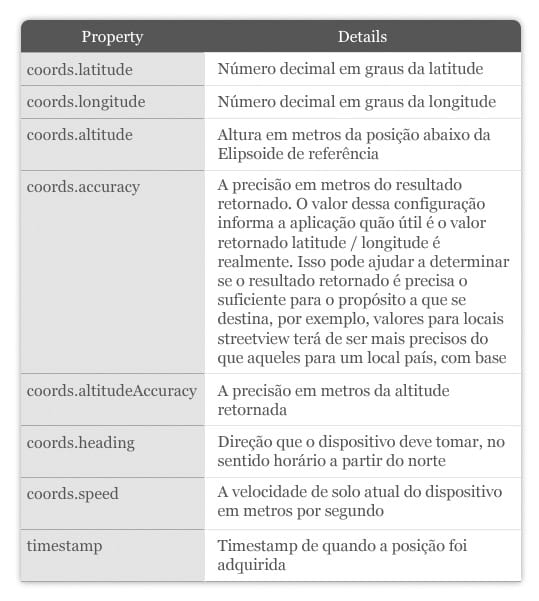
\includegraphics[width=0.8\textwidth]{./dados/figuras/fig1}
    \fonte{\citeonline{oficinanetagps:2018}}
    \label{fig:figura-propertycoords}
\end{figure}

\section{A-GPS}
O Sistema de Posicionamento Global Assistido, desenvolvido para localizar satélites com mais rapidez e confiabilidade, dispõe de recursos de rede para localizar e utilizar os satélites em condições de sinal fraco. É uma versão otimizada do  GPS, que recebe dados através de uma conexão de dados (GPRS ou 3G), permitindo que o aparelho calcule as coordenadas da sua posição atual ao receber informações satelitais, sob certas condições, como pode ser visto na \autoref{fig:figura-funcagps} \cite{oficinanetagps:2018}. 

\begin{figure}[H]
    \centering
    \caption{Funcionamento do A-GPS}
    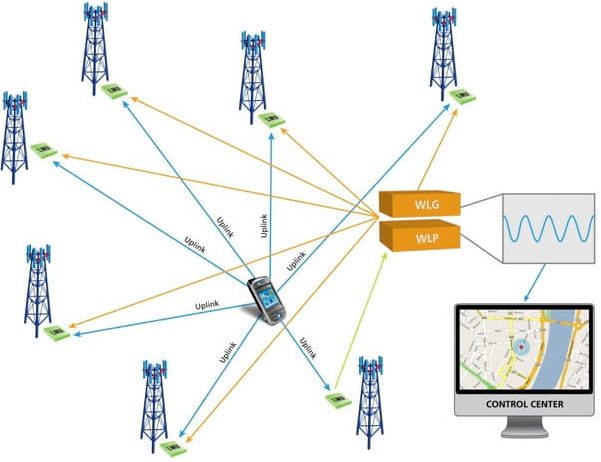
\includegraphics[width=1.0\textwidth]{./dados/figuras/fig2}
    \fonte{\citeonline{oficinanetagps:2018}}
    \label{fig:figura-funcagps}
\end{figure}

%%% Original: Esta tecnologia se torna superior a sua antecessora devido a precisão e disponibilidade das coordenadas do dispositivo em tempo real, apesar dos custos cobrados pela transferência de dados sobre a rede celular pela operadora utilizada, não sofrendo alterações de propagação \textit{multipath} (caminhos secundários que o sinal percorre até chegar à antena do receptor, como mostrado na \autoref{fig:figura-propagmultipath}), como por exemplo, de construções, ruas, edifícios, rios, lagos, veículos ou condições atmosféricas \cite{oficinanetagps:2018} \cite{multicaminho:2004}.

Esta tecnologia se torna superior a sua antecessora devido a melhora de precisão e disponibilidade das coordenadas do dispositivo em tempo real, apesar dos custos cobrados pela transferência de dados sobre a rede celular pela operadora utilizada. Este sistema não sofre alterações de propagação \textit{multipath} (caminhos secundários que o sinal percorre até chegar à antena do receptor, como mostrado na \autoref{fig:figura-propagmultipath}), como por exemplo, de construções, ruas, edifícios, rios, lagos, veículos ou condições atmosféricas \cite{oficinanetagps:2018} \cite{multicaminho:2004}.

 A maior utilidade do sistema de A-GPS se faz em áreas urbanas, repletas de desfiladeiros urbanos, melhorando a experiência do usuário para todos os aplicativos que usam o GPS integrado e reduzindo o tempo que um aparelho com GPS leva para localizar a sua posição atual, conhecido como TTFF (Tempo de Localização Inicial) \cite{oficinanetagps:2018}.

\begin{figure}[H]
    \centering
    \caption{O problema do multipath}
    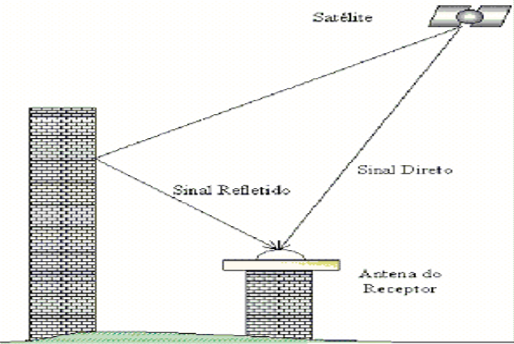
\includegraphics[width=0.7\textwidth]{./dados/figuras/fig3}
    \fonte{\citeonline{multicaminho:2004}}
    \label{fig:figura-propagmultipath}
\end{figure}

\subsection{Diferenças entre GPS e A-GPS}

%%% Original: O GPS inicialmente realiza uma busca por satélites disponíveis para auxiliá-lo na navegação, ao encontrar o primeiro satélite disponível, o aparelho recebe informações sobre a localização dos outros satélites próximos, iniciando a roteirização da localização atual do mesmo. Este processo é demorado, devido à lenta conexão GPS entre os satélites ser muito lenta.

Inicialmente o GPS realiza uma busca por satélites disponíveis para auxiliá-lo na navegação. Quando o GPS encontra o primeiro satélite disponível, o aparelho recebe informações sobre a localização dos outros satélites próximos, iniciando a roteirização da localização atual do mesmo. Este processo é demorado, pelo fato de que a conexão GPS entre os satélites é muito lenta.

%%% Original: Para dispositivos A-GPS, são utilizados servidores, como por exemplo uma torre de redes móvel (antenas de celulares) e bases (servidores) para obter as informações dos satélites constantemente. Uma vez que esses servidores estão continuamente enviando e recebendo informações dos satélites, não há atraso em demorar a conhecer a órbita e a localização exata dos satélites, o tempo para o recebimento dos dados é muito mais rápido que um GPS normal, já que os dados já estão armazenados nos servidores, que analisam os sinais fragmentados recebidos do receptor GPS e aqueles recebidos diretamente do satélite para corrigir erros, proporcionando uma localização exata do aparelho, onde o mesmo só precisará realizar alguns cálculos de triangulação com as antenas de redes móveis por final.

Para dispositivos A-GPS, são utilizados servidores, como por exemplo uma torre de rede móvel (antenas de celulares) e bases (servidores) para obter as informações dos satélites constantemente. Uma vez que esses servidores estão continuamente enviando e recebendo informações dos satélites, não há atraso para conhecer a órbita e a localização exata dos satélites. O tempo para o recebimento dos dados é muito mais rápido que um GPS normal, já que os dados já estão armazenados nos servidores, que analisam os sinais fragmentados recebidos do receptor GPS e aqueles recebidos diretamente do satélite para corrigir erros, proporcionando uma localização exata do aparelho, onde o mesmo só precisará realizar alguns cálculos de triangulação com as antenas de redes móveis por final \cite{oficinanetagps:2018}.

Ainda conforme o autor citado acima, a conexão inicial é feita com uma antena de telefonia celular que previamente armazenou a localização destes satélites e as transmite para o aparelho com uma velocidade até 40 vezes maior. Este recurso só é possível em aparelhos com conexão GPRS, caso este sinal esteja devido à regiões cercadas por edifícios muito altos, o A-GPS utiliza o apoio da antena quando o sinal GPS, ajudando a manter o sinal estável. Não existindo cobertura de celular, o aparelho funcionará normalmente como um GPS convencional. O uso do A-GPS se torna a utilização mais eficaz, evitando o aguardo pela conexão entre satélites. Na \autoref{fig:figura-localizacaoGpsAgps} é possível visualizar como é feita a localização GPS e A-GPS.

\begin{figure}[H]
    \centering
    \caption{Localização GPS e A-GPS}
    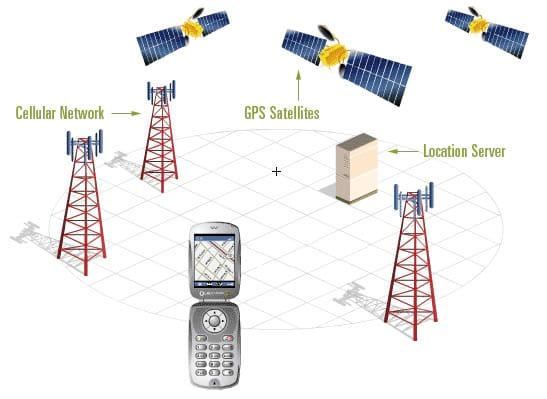
\includegraphics[width=0.8\textwidth]{./dados/figuras/fig5}
    \fonte{\citeonline{oficinanetagps:2018}}
    \label{fig:figura-localizacaoGpsAgps}
\end{figure}

\section{Google Maps}

%%% Original: O Google Maps é um dos recursos da Google mais popular de todos, amplamente utilizado por aqueles que querem se garantir na hora de chegar a um local desconhecido. Além de oferecer o serviço de mapas, o software inclui outras características muito úteis, como ferramentas para calcular as direções entre dois pontos. Pode-se obter mais informações sobre qualquer lugar, graças à utilização de fotos, \textit{webcams} e artigos. Seja pelos seus recursos básicos, como encontrar endereços específicos e verificar trajetos e distâncias entre dois ou mais pontos, ou pelos avançados, como a visão de satélite e o Street View, ele se destaca com facilidade neste mercado. Em parte graças à sua enorme abrangência, poucas cidades e ruas ainda não estão nele, permitindo fazer o \textit{download} de uma área no dispositivo para ser usado sem conexão com a internet, através das áreas \textit{off-line}. Os mapas salvos dessa forma são renovados a cada 30 dias por meio de redes \textit{Wi-Fi}, caso o usuário fique mais de 30 dias sem usá-los, o aplicativo sugerirá que ele renove a área ou a apague para economizar espaço. Esse recurso é especialmente útil para viagem à outro país e sem plano de dados móveis \cite{google:2019}. Na \autoref{fig:figura-googlemaps} pode-se ver um exemplo de visualização de mapa do Google Maps.

%%% Rev-Madalozzo: "mais popular de todos" não é uma frase interessante. O que são todos? Quem define se é popular ou não?
O Google Maps é uma aplicação fornecida pela Google amplamente utilizada por aqueles que necessitam de auxílio para chegar a um local desconhecido. Além de oferecer o serviço de mapas, o software inclui outras características muito úteis, como as ferramentas para calcular as direções entre dois pontos. Pode-se obter mais informações sobre qualquer lugar, graças à utilização de fotos, \textit{webcams} e artigos. Seja pelos seus recursos básicos, como encontrar endereços específicos e verificar trajetos e distâncias entre dois ou mais pontos, ou pelos avançados, como a visão de satélite e o Google Street View, ele se destaca com facilidade neste mercado. Em parte, graças à sua enorme abrangência, poucas cidades e ruas ainda não estão mapeadas neste serviço, permitindo fazer o \textit{download} de uma área no dispositivo para ser usado sem conexão com a internet. Os mapas salvos dessa forma são renovados a cada 30 dias por meio de redes \textit{Wi-Fi}, caso o usuário fique mais de 30 dias sem usá-los, o aplicativo sugerirá que ele renove a área ou a apague para economizar espaço. Esse recurso é especialmente útil para viagem à outro país e sem plano de dados móveis \cite{google:2019}. Na \autoref{fig:figura-googlemaps} pode-se ver um exemplo de visualização de mapa do Google Maps.

\begin{figure}[H]
    \centering
    \caption{Exemplo de visualização do Google Maps}
    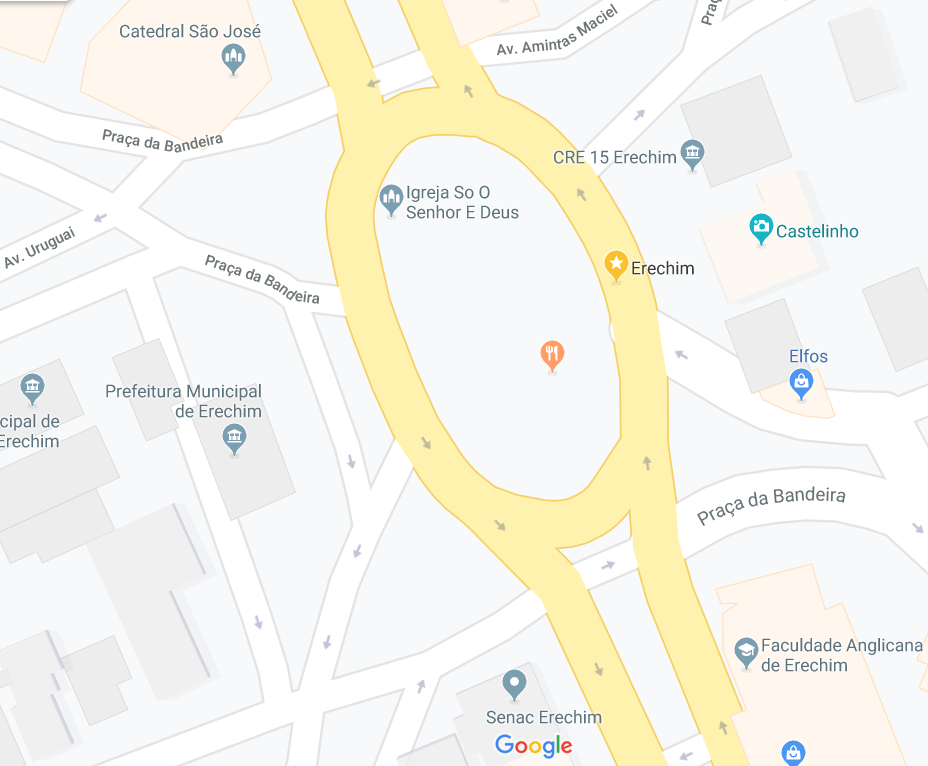
\includegraphics[width=0.9\textwidth]{./dados/figuras/fig4}
    \fonte{\citeonline{googleMaps:2019}}
    \label{fig:figura-googlemaps}
\end{figure}

%%% Original: A principal utilização é a busca por endereços, a partir de um computador, independentemente do navegador e do sistema operacional, basta digitar o endereço que deseja encontrar. Além de digitar o local manualmente, é possível indicá-lo diretamente no mapa. Também é possível descobrir novos locais, como lojas, restaurantes entre outros pontos de interesse facilmente, através de categorias e subcategorias, como “para ir com crianças” e “para gastar pouco”. Tudo isso, são locais escolhidos com base na localização atual e que se adaptam ao gosto de cada usuário. É comum ser disponibilizado mais de um caminho para o destino final, exibindo por padrão a mais rápida, levando em consideração a variação de trânsito para o horário atual. Isso é possível porque o Google Maps acumula informações sobre o tráfego da região. Ou seja, ele sabe qual é o fluxo de veículos para um determinado local em um determinado horário. Além de encontrar qualquer localidade, demonstrar informações meteorológicas ou indicações e caminhar ao redor das cidades mais importantes do globo, é um de seus diferenciais \cite{google:2019}.

Segundo dados da Google, a principal utilização realizada no Google Maps é a busca por endereços. A partir de um computador, independentemente do navegador e do sistema operacional, basta digitar o endereço que deseja encontrar. Além de digitar o local manualmente, é possível indicá-lo diretamente no mapa. Também, é possível descobrir novos locais, como lojas, restaurantes entre outros pontos de interesse facilmente, através de categorias e subcategorias, como “para ir com crianças” ou “para gastar pouco”. Tudo isso, são locais escolhidos com base na localização atual e que se adaptam ao gosto de cada usuário. É comum ser disponibilizado mais de um caminho para o destino final, exibindo por padrão a mais rápida, levando em consideração a variação de trânsito para o horário atual. Isso é possível porque o Google Maps acumula informações sobre o tráfego da região. Ou seja, ele sabe qual é o fluxo de veículos para um determinado local em um determinado horário. Além de encontrar qualquer localidade, demonstrar informações meteorológicas ou indicações e caminhar ao redor das cidades mais importantes do globo, é um de seus diferenciais \cite{google:2019}.

%%% Original: Para ajudar quem andar de ônibus, metrô e trem pelas cidades do mundo, é possível saber a melhor rota de transporte público, qual o ponto de ônibus mais perto e os pontos de parada do coletivo. Dispondo de serviços de altitude para ciclistas, é possível identificar as variações do terreno em metros durante o trajeto, além de levar em conta a estrutura cicloviária da cidade. Às vezes, esse caminho pode nem ser o mais direto entre os dois pontos, mas ele pretende ser o mais seguro e agradável para quem está pedalando \cite{google:2019}.

Para ajudar quem anda de ônibus, metrô e trem pelas cidades do mundo, é possível saber a melhor rota de transporte público, qual o ponto de ônibus mais perto e os pontos de parada do coletivo. Dispondo de serviços de altitude para ciclistas, é possível identificar as variações do terreno em metros durante o trajeto, além de levar em conta a estrutura cicloviária da cidade. Às vezes, esse caminho pode nem ser o mais direto entre os dois pontos, mas ele pretende ser o mais seguro e agradável para quem está pedalando \cite{google:2019}.

Com uma enorme base de dados, serviços como Booking, Decolar ou Kayak, podem ser encontrados ao pesquisar por um hotel na plataforma da Google, contando com uma ferramenta interna para ajudar seus usuários, que apresentam diversas opções de quartos vagos na região, com o preço médio. Caso o local de visita escolhido durante uma viagem seja bem conhecido, é possível fazer um \textit{tour} pelo espaço interno mapeado. No Maracanâ, por exemplo, é possível visualizar a divisão das arquibancadas. O plano da empresa é estender esse recurso a outros estabelecimentos de grande porte, como parques e shoppings. Muitas das opções de uso citadas fazem parte da Google Street View, que mapeia locais possíveis de caminhar virtualmente por várias cidades ao redor do mundo, podendo encontrar exatamente a fachada do local desejado. Além do Google Earth e dos Indoor Maps, o Google Maps traz também outra função capaz explorar o mundo a partir da tela do computador chamada Google Treks, desenvolvido para visitar virtualmente alguns lugares incríveis da Terra.

Selecionando a cidade de partida e a cidade de chegada e o meio de transporte ''Avião'', faz o Google Maps exibir informações de voos disponíveis para o trajeto, é possível obter informações relacionadas a duração do voo e quais companhias aéreas operam aquele trajeto \cite{google:2019}. 

O recurso mais recente adicionado a plataforma, permite planejar uma rota com \textit{waypoints}. É a possibilidade de fazer percursos que incluam diversas parada, indicando o melhor caminho do ponto A até B, e depois de B até C, sem precisar mudar a rota novamente, muito usado para encontrar o melhor caminho para visitar diversos pontos turísticos de uma cidade no mesmo dia.

Várias ferramentas de visualização geoespacial dos principais \textit{players} da indústria da internet estão tomando o mundo digital. Google, Yahoo, Microsoft e Amazon lançaram ferramentas de mapeamento baseada em geolocalização e, coletivamente, elevaram o nível de mapeamento da internet. Por mais que suas capacidades funcionais não forneçam nada de muito diferente do que fornecedores tradicionais da GIS (\textit{Geographic Information System}) já tinham, o surgimento destes serviços foi significativo na medida em que conseguiram captar um público mais amplo. O Google entrou como líder destes serviços com seu produto Google Maps, que fornece uma interface visual atrativa, construídas com tecnologia AJAX, além de dados detalhados de imagens aéreas da superfície terrestre, e uma API aberta que permite a personalização do mapa, incluindo a capacidade de adicionar dados específicos ao mapa e traçar rotas \cite{geospatial:2009}.

\subsection{Google Maps Platform}

A plataforma para desenvolvedores da Google se chama Google Maps Platform, onde 99\% de cobertura no mundo, com a abrangência de mais de 200 países e territórios, estão disponíveis. Contemplando informações de local precisas e em tempo real, são mais de 25 milhões de atualizações por dia e 1 bilhão de usuários ativos por mês, tudo isso gerando uma grande base de dados para consulta \cite{google:2019}. Nela, se obtêm soluções para cada setor:
\begin{itemize}
    \item Serviço de transporte particular: disponibiliza a integração com qualquer aplicativo de serviço de transporte particular para diminuir os tempos de espera dos clientes e os erros de navegação dos motoristas;
    \item Jogos: permite criar jogos imersivos e realistas com milhões de estruturas em 3D personalizáveis, dados globais atualizados e integração perfeita com o Unity;
    \item Rastreamento de recursos: possibilita maior eficiência na localização de veículos e os recursos em tempo real, visualizando o trajeto dos mesmos e orientando os motoristas durante viagens complexas. 
\end{itemize}

\subsubsection{Maps}

O recurso Maps presente na Google Maps Platform, leva o mundo real até os usuários por meio de mapas estáticos e dinâmicos, imagens do Google Street View e visualizações 360º, visualizando o mundo com mapas eficientes e precisos, podendo ser incorporado em sites ou aplicativos. O Street View e as imagens de satélite permitem  trabalhar com personalizações e sobreposições capazes de se adequar com a necessidade de cada usuário, com uma infraestrutura está sempre disponível para ampliação \cite{google:2019}. 

\subsubsection{Routes}

Através de dados abrangentes e trânsito em tempo real, encontrar o melhor caminho até o destino final se torna um trabalho rápido com o uso do recurso denominado ''Routes''. Com informações de navegação confiáveis e mais de 64 milhões de quilômetros de estradas em todo o mundo, traçar percursos entre cidades ou encontrar hotéis, permite maior eficiência, redução de custos e melhorar a experiência dos clientes finais. Este recurso permite planejar viagens munido de dados atualizados sobre a distância entre pontos, trajetos sugeridos e tempos estimados de deslocamento, com a capacidade de criar trajetos eficientes para até 25 pontos de referência, agilizando os sistemas de entrega, criando itinerários para turistas ou guiar os clientes que alugam carros do seu escritório até os hotéis, realocando o mesmo caso o caminho escolhido possua tráfego \cite{google:2019}. Sua eficiência é justificada pelo agrupamento dos seguinte recursos:

\begin{itemize}
    \item \textit{Directions}: fornece rotas de transporte público, bicicleta, carro e a pé, calcula os tempos de deslocamento atuais ou futuros com base no trânsito em tempo real;
    \item \textit{Distance Matrix}: calcula tempos de deslocamento e distâncias para um ou mais locais;
    \item \textit{Roads}: permite criar itinerários precisos determinando o trajeto percorrido pelo veículo e as vias mais próximas ao longo de cada ponto da viagem do veículo.
\end{itemize}

\subsubsection{Places}

Contempla informações avançadas de mais de 150 milhões de pontos de interesse, permitindo encontrar locais específicos por meio de números de telefone, endereços e sinais em tempo real. Com usuários atualizando a todo momento, 24 horas por dia, as avaliações medidas pela Google se tornam confiantes, capazes de planejar uma viagem ou indicar um restaurante através dos gostos dos usuários. Com o Places, é possível compartilhar detalhes sobre nomes de locais, endereços, classificações, comentários, dados de contato e ambiente. Os Local Guides e os usuários enviam milhões de atualizações todos os dias \cite{google:2019}. Este recurso é o maior agrupador de todos, abrange:

\begin{itemize}
    \item \textit{Place Details}: fornece nomes, endereços e outros detalhes valiosos, como classificações, avaliações ou dados de contato de pontos de interesse;
    \item \textit{Current Place}: identifica um local com base nos sinais em tempo real, como hora do dia ou local;
    \item \textit{Find Place}: localiza usando o número de telefone, endereço ou nome do local;
    \item \textit{Automatic Filling}: sugere informações de local enquanto os usuários digitam;
    \item \textit{Geocoding}: converte endereços em coordenadas geográficas e vice-versa;
    \item \textit{Geolocation}: captura o local preciso de um dispositivo usando o \textit{Wi-Fi} ou torres de celular como base;
    \item \textit{Time Zone}: mostra o fuso horário de qualquer local.
\end{itemize}